\documentclass{article}
\usepackage[dvipsnames]{xcolor}
\usepackage[colorlinks=true,citecolor=blue]{hyperref}
\usepackage{amsmath}
\usepackage{pgfplots}
\usetikzlibrary{
		calc,
		patterns,
		positioning
	}
\pgfplotsset{
		compat=1.18,
		samples=30,
		clip=false,
		my axis style/.style={
			axis x line=middle,
			axis y line=middle,
			legend pos=outer north east,
			axis line style={->},
			legend style={font=\footnotesize},
			label style={font=\footnotesize},
			tick label style={font=\footnotesize},
			xlabel style={at={(ticklabel* cs:1)},anchor=west,font=\footnotesize},
			ylabel style={at={(ticklabel* cs:1)},anchor=west,font=\footnotesize},
			xlabel=$X$,
			ylabel=$Y$
		},
	}
\tikzset{
		>=stealth
	}

\newcommand{\E}{\mathrm{e}}

\begin{document}

	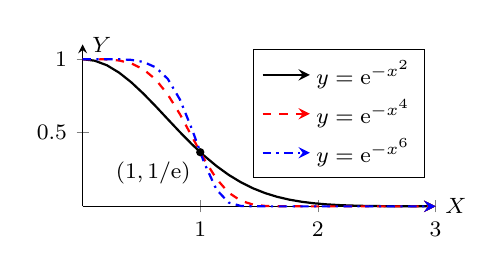
\begin{tikzpicture}
	   \begin{axis}[
		my axis style,
		width=.5\textwidth,
		height=.3\textwidth,
        ymax = 1.1,
		legend entries={$y = \E^{-x^2}$, $y = \E^{-x^4}$, $y = \E^{-x^6}$},
		legend pos=north east
	    ]

	    \addplot[domain=0:3, thick, ->]
	    {exp(-(x)^2)};

	    \addplot[domain=0:3, thick, red, dashed, ->]
	    {exp(-(x)^4)};

	    \addplot[domain=0:3, thick, blue, dashdotted, ->]
	    {exp(-(x)^6)};

	    \fill[black]
	    (1,.36788) circle (1.5pt) node[below left] {\footnotesize $(1, 1/\E)$};

	   \end{axis}
	\end{tikzpicture}

\end{document}